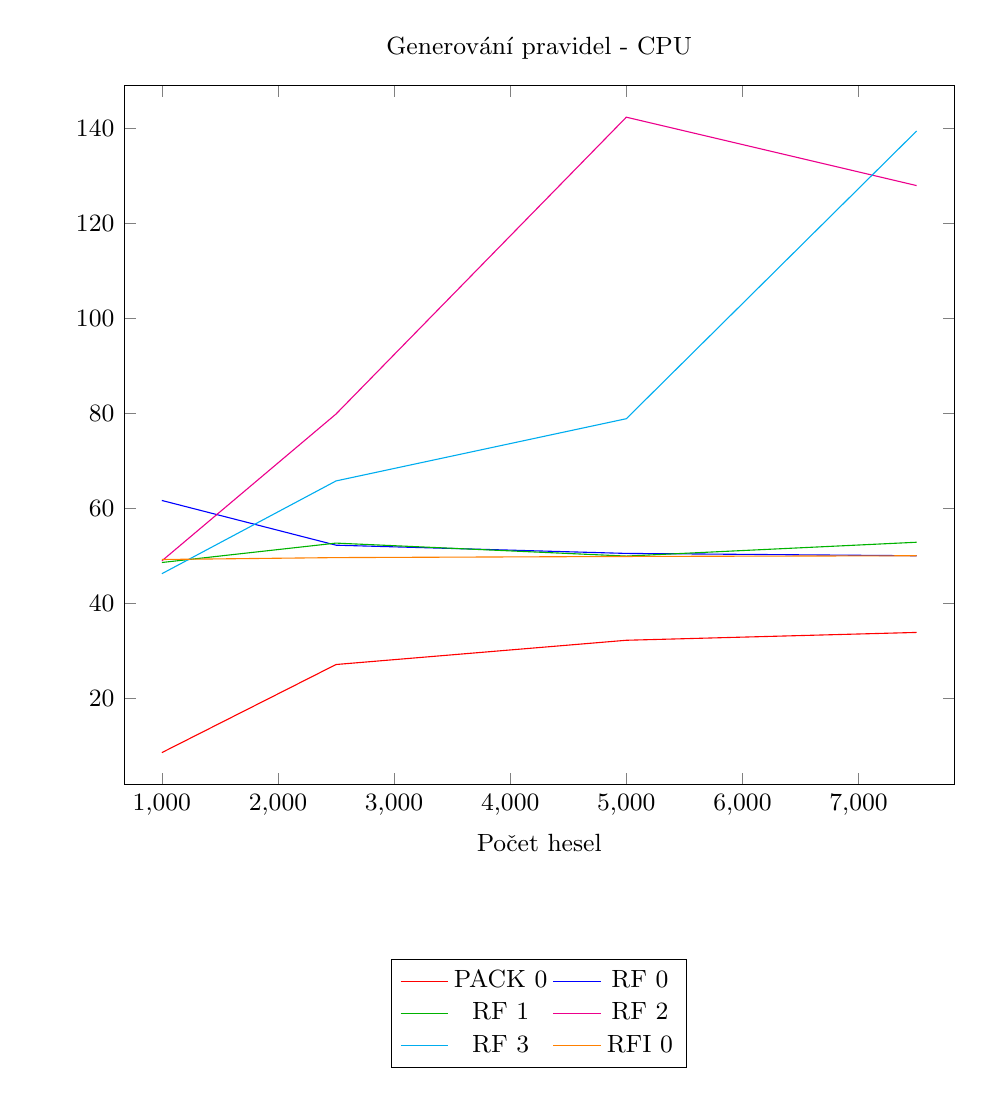
\begin{tikzpicture}
  \begin{axis}[
    width=\linewidth, 
    every axis/.append style={font=\small},
    title={Generování pravidel - CPU},
    xlabel={Počet hesel},
    ylabel={\phantom{Průměr CPU v \%}},
    legend style={
      at={(0.5,-0.25)},
      anchor=north,
      legend columns=2,
    },
    enlargelimits=0.05,
    scaled y ticks = false,
    scaled x ticks = false,
    cycle list={
     {red},
     {blue},
     {green!70!black},
     {magenta},
     {cyan},
     {orange},
     {violet},
     {purple},
     {gray},
     {darkgray}%
    }
    ]
    
    \addplot coordinates {
      (1000, 8.66) 
      (2500, 27.19) 
      (5000, 32.29) 
      (7500, 33.94) 
      }; % PACK 0
    
    \addplot coordinates {
      (1000, 61.7) 
      (2500, 52.29) 
      (5000, 50.56) 
      (7500, 50.07) 
      }; % RF 0
    
    \addplot coordinates {
      (1000, 48.65) 
      (2500, 52.73) 
      (5000, 50.0) 
      (7500, 52.91) 
      }; % RF 1
    
    \addplot coordinates {
      (1000, 48.99) 
      (2500, 79.89) 
      (5000, 142.33) 
      (7500, 127.94) 
      }; % RF 2
    
    \addplot coordinates {
      (1000, 46.29) 
      (2500, 65.81) 
      (5000, 78.9) 
      (7500, 139.42) 
      }; % RF 3
    
    \addplot coordinates {
      (1000, 49.28) 
      (2500, 49.68) 
      (5000, 49.92) 
      (7500, 50.07) 
      }; % RFI 0
    
    \legend{PACK 0, RF 0, RF 1, RF 2, RF 3, RFI 0}
  \end{axis}
\end{tikzpicture}